\documentclass[]{article}

\usepackage[margin=1.0in]{geometry}
\usepackage{amsmath}
\usepackage{amsfonts}
\usepackage{amsthm}
\usepackage{graphicx}
\usepackage{amssymb}

\usepackage{mathtools}

%opening
\title{Computing the Hausdorff Dimension for Symmetric Schottky Groups}
\author{Alex Karlovitz}
\date{}

\begin{document}
	
	\maketitle
	
\section*{Schottky Groups in the Unit Disk}

We can form a Schottky group in the unit disk as follows:
let $\mathcal{C}$ be a finite collection of disjoint circles which are orthogonal to the unit circle (actually, we will allow two circles in $\mathcal{C}$ to be tangent, so their intersections with the open unit disk are disjoint).
Then the group $\Gamma(\mathcal{C})$ generated by reflections across these circles in the unit disk is an example of a \textit{Schottky group}.

\subsection*{Example: Symmetric Circles}

A simple example of a Schottky group in the unit disk is obtained by taking circles of the same size spaced symmetrically about the disk.
We could parameterize such sets of circles by the two variables $n$ and $\theta$, where $n$ is the number of circles and $\theta$ is the angle along the unit circle cut out by one of the circles.
See Figure \ref{pi_over_2} for an example.

\begin{figure}[h]
	\centering
	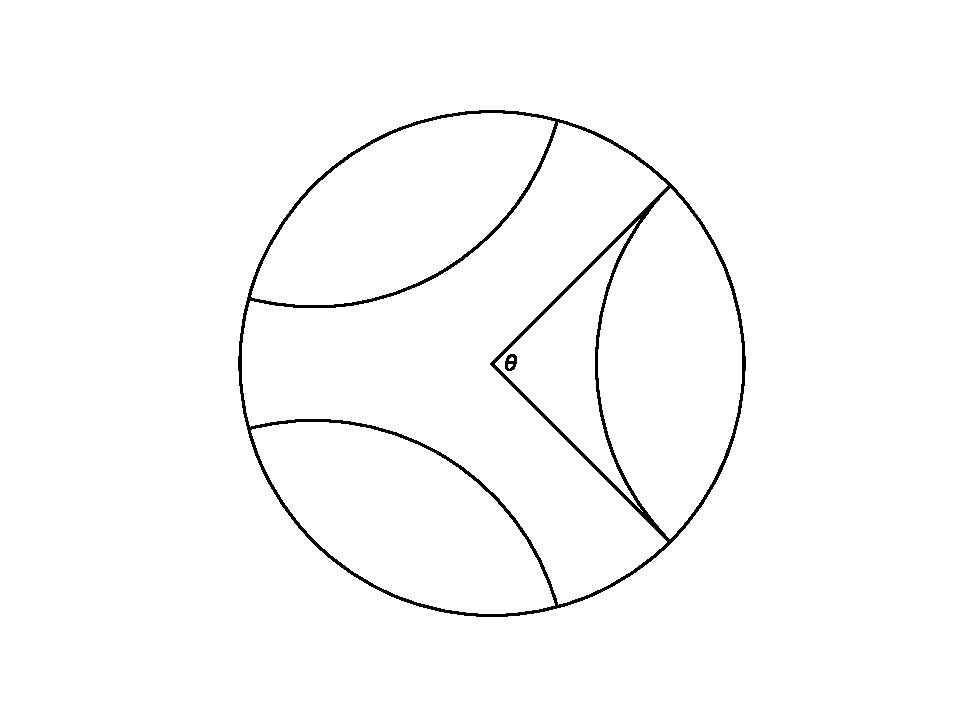
\includegraphics[trim=110 40 100 50, clip, width=0.6\linewidth]{pi_over_2.pdf}
	\caption{Example with $n = 3$ circles cutting out arcs of angle $\theta = \frac{\pi}{2}$}
	\label{pi_over_2}
\end{figure}

A fundamental domain for such a Schottky group is the exterior of all the circles (inside the unit disk of course).
To see this, label the reflections across the $n$ circles $R_1, \dots, R_n$.
We will also use $R_i$ to denote the actual reflections; the meaning should be clear from context.
Let
$$
\gamma = R_{i_1}\cdots R_{i_k}
$$
be a reduced word of length $k$ in the reflections (by \textit{reduced} we mean that $R_{i_j} \neq R_{i_{j+1}}$ for all $j$, since reflections are involutions).
Note that every element of the Schottky group can be written as such a reduced word.
Now suppose $z$ is any element of the fundamental domain.
If $k = 1$, then it is clear that $\gamma(z)$ is inside the circle $R_{i_1}$.
By induction, it is then easy to see that for $k \geq 1$, $\gamma(z)$ is always in the circle $R_{i_1}$.
Thus, the only way for $\gamma(z)$ to be in the fundamental domain is t o have $k = 0$; i.e., $\gamma$ is the identity.

To see that every orbit has a point in the fundamental domain, one must check that given a point in one of the circles $R_i$, reflection through that circle \textit{decreases} the distance from the point to $0$.
Thus, since the Schottky group acts discretely on hyperbolic space, we can eventually move any point to the fundamental domain by repeatedly reflecting outside of any circle it falls in.

See Figure \ref{disk_FD} for an example.

\begin{figure}[h]
	\centering
	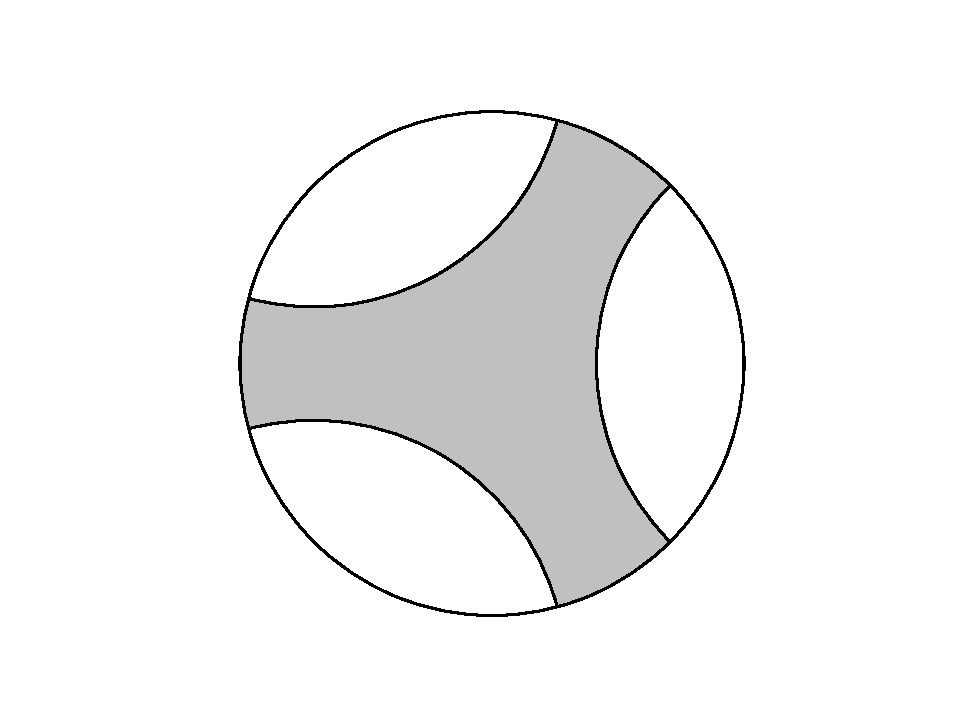
\includegraphics[trim=110 40 100 50, clip, width=0.6\linewidth]{disk_FD.pdf}
	\caption{The example from Figure \ref{pi_over_2} with a fundamental domain filled in.}
	\label{disk_FD}
\end{figure}

\textbf{Note:} For the rest of the document, we will focus on the case $n = 3$.
The discussion extends easily to $n > 3$.

\section*{Rotational Symmetry of Maass Forms}

Recall that Maass forms for $\Gamma$ are eigenfunctions of the Laplace-Beltrami operator acting on $L^2(\Gamma\backslash\mathbb{H})$.
We claim that for a given eigenvalue, a Maass form for the symmetric Schottky group of parameters $(n, \theta)$ can be taken to be invariant under rotation by $2\pi/n$.
\\

To verify this claim, first recall that the Laplace operator on the disk model (in polar coordinates) is
$$
\Delta = -\left(\frac{(1 - \rho^2)^2}{4}\frac{\partial^2}{\partial\rho^2} +
\frac{(1 - \rho^2)^2}{4\rho}\frac{\partial}{\partial\rho} +
\frac{(1 - \rho^2)^2}{4\rho^2}\frac{\partial^2}{\partial\theta^2}\right)
$$
From this formula, one easily sees that rotations are $\Delta$-invariant.
Thus, if we compose any eigenfunction of the Laplacian with a rotation, we still have an eigenfunction of the same eigenvalue.

Next, note that a rotation of $2\pi/n$ is smooth on the fundamental domain for the $(n, \theta)$ symmetric Schottky group.
Thus, given a Maass form $f$, we can construct a $2\pi/n$ rotation-invariant Maass form of the same eigenvalue by taking the linear combination
$$
\frac{1}{n}\sum_{i = 0}^{n - 1}f\left(e^{2\pi i/n} z\right)
$$

So we can assume that any Maass form we are working with is invariant under rotation by $2\pi/n$.
Even further, we can use the multiplicity one principle to conclude that the base eigenfunction is itself invariant under this rotation.

\subsection*{Consequences for Hejhal's Algorithm}

When running Hejhal's algorithm on the symmetric Schottky groups, we need only consider test points in one $2\pi/n$ sector.
We can of course take this sector to entirely contain one flare, while not intersecting any others.

If the pullback $z^*$ of a test point $z$ falls outside of the chosen sector, we can simply replace $z^*$ with the appropriate rotation to make it fall in this sector, since the Maass form will be equivalent at those different points.
\\

In a previous iteration of this work, we went through what this means for choosing test points for Hejhal's algorithm.
One finds that the only admissible points come from a very specific area in a flare domain.
Unfortunately, these test points end up giving very slow convergence in the flare expansion, thus making them useless for Hejhal's algorithm.

These considerations lead one to consider looking at covers of the Schottky group, perhaps by building the rotational invariance into the group itself.
We consider this idea in the next section.

\section*{On Covers of the Symmetric Schottky Group}

In this section, we assume we are interested in a symmetric Schottky group with three circles.
We will construct another group which contains the Schottky group as a finite index subgroup.
Because it is a finite degree cover, it will share its bottom eigenvalue with the Schottky group.
Moreover, our cover will admit a doubling which comprises only of M\"obius transformations, making it more suitable for use in Hejhal's algorithm.
Finally, the hope is that the larger group (with a smaller fundamental domain) will allow for a greater variety of admissible test points.

\subsection*{A Larger Reflection Group}

We begin by considering a reflection group which contains our symmetric Schottky group as a proper subset.
We will describe this group in the disk model.
We define three geodesics by stating their endpoints:
\begin{itemize}
	\item $D_1$ connects -1 and 1
	\item $D_2$ connects $-e^{i\pi/3}$ and $e^{i\pi/3}$
	\item $R$ connects $e^{-i\theta}$ and $e^{-\theta}$
\end{itemize}
where $\theta$ is the parameter for our symmetric Schottky group.
Let $\Gamma$ be the group generated by the reflections through these geodesics.
$$
\Gamma = \langle D_1, D_2, R \rangle
$$
(Note that we are abusing notation and letting $D_1, D_2$, and $R$ refer to the reflection through the corresponding geodesics).
See Figure \ref{fd_reflection} for an example with $\theta = \pi/2$.
\begin{figure}
	\centering
	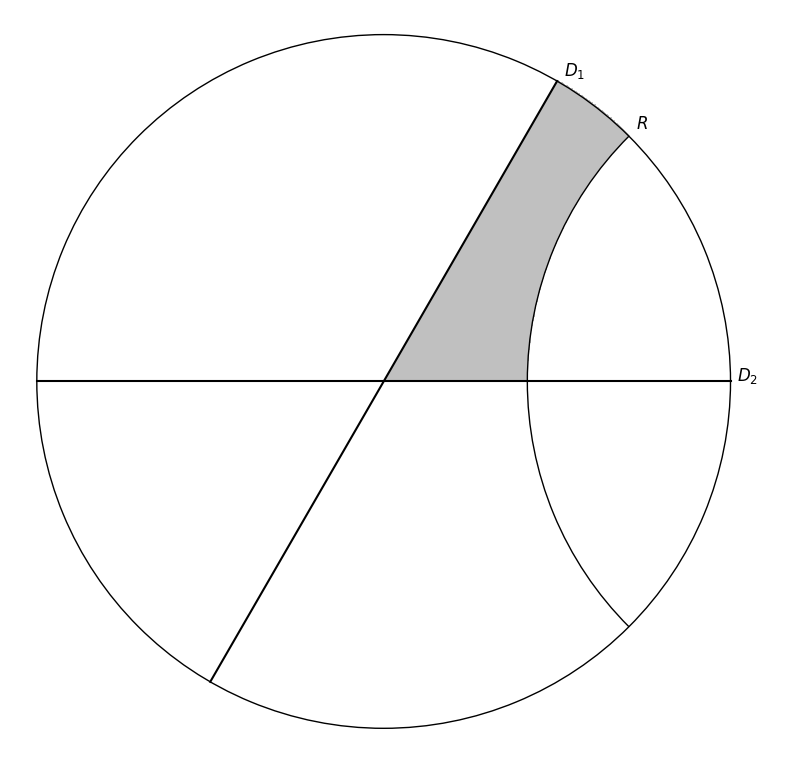
\includegraphics[width=0.5\linewidth]{reflection_group.png}
	\caption{Fundamental Domain for $\Gamma$ with $\theta = \pi/2$}
	\label{fd_reflection}
\end{figure}

To see that $\Gamma$ contains our Schottky group, first observe that the composition $S = D_1D_2$ is just rotation by $2\pi/3$.
Thus, $S(R)$ and $S^2(R)$ give the other two circles in the Schottky group.
In particular, $S^{-1}RS$ and $SRS^{-1}$ give the reflections through those two circles.
Thus, all three generators of the symmetric Schottky group are contained in $\Gamma$.

\subsection*{Doubling Across $D_1$}

The group $\Gamma$ will have the same bottom eigenvalue as the symmetric Schottky group; however, since $\Gamma$ is a reflection group, it contains elements which are not M\"obius transformations.
To rectify this, we will double the group across $D_1$.
Since a composition of two reflections is a M\"obius transformation, the doubled group will comprise solely of these.
Moreover, doubling a group does not affect its bottom eigenvalue, so we will still be able to study the doubled group when applying Hejhal's algorithm to discover the base eigenvalue for the symmetric Schottky group.

Specifically, we are looking at the group
$$
\Gamma_0 = \langle D_1D_2, D_1R \rangle
$$
This is called \textit{doubling} across $D_1$ since the fundamental domain for the doubled group is exactly the old fundamental domain plus its reflection across $D_1$ (see Figure \ref{fd_reflection_doubled}).
\begin{figure}
	\centering
	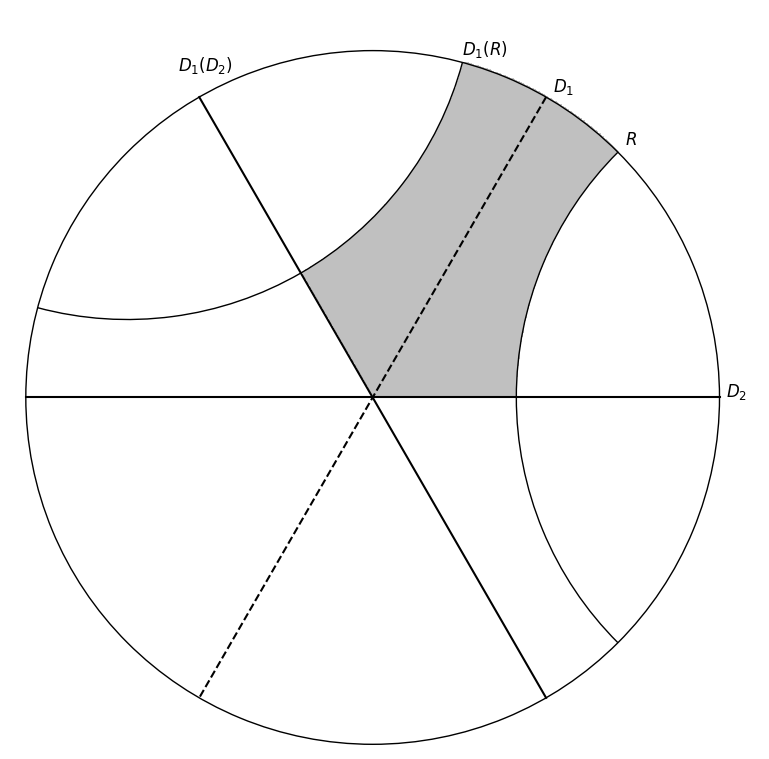
\includegraphics[width=0.5\linewidth]{reflection_doubled.png}
	\caption{Fundamental Domain for $\Gamma_0$ with $\theta = \pi/2$}
	\label{fd_reflection_doubled}
\end{figure}
Note that the composition $D_1D_2$ is just rotation by angle $2\pi/3$.
It will be necessary to also determine the action of another generator.
To simplify this, we first note that we can replace $D_1R$ with $(D_1D_2)^{-1}D_1R = D_2R$ as a generator.
This is helpful since the action of $D_2$ is simply conjugation.
Next, we note that the circle containing the geodesic $R$ has center $\sec(\theta/2)$ and radius $\tan(\theta/2)$.
Thus, reflection through $R$ can be written as
$$
R(z) = \frac{\tan^2(\theta/2)}{\bar{z} - \sec(\theta/2)} + \sec(\theta/2)
$$
We can now explicitly write down the action of $D_2R$.
$$
D_2R(z) = \overline{R(z)} =
\frac{\sec(\theta/2)z - 1}{z - \sec(\theta/2)}
$$
One notices that multiplying the numerator and denominator by $i\cot(\theta/2)$ converts this to a M\"obius transformation where the corresponding matrix is in $\text{PSU}(1, 1)$ (this is the matrix group which is conjugate via the Cayley transform to $\text{PSL}(2, \mathbb{R})$).
Specifically,
$$
D_2R(z) = \frac{i\csc(\theta/2)z - i\cot(\theta/2)}{i\cot(\theta/2)z - i\csc(\theta/2)}
$$
In this way, we see that $\Gamma_0 = \langle D_1D_2, D_2R \rangle$ is isomorphic to the matrix group
$$
\left\langle
\begin{pmatrix}
e^{i\pi/3} & ~ \\
~ & e^{-i\pi/3}
\end{pmatrix},
\begin{pmatrix}
i\csc\frac{\theta}{2} & -i\cot\frac{\theta}{2} \\
i\cot\frac{\theta}{2} & -i\csc\frac{\theta}{2}
\end{pmatrix}
\right\rangle < \text{SU}(1, 1)
$$

\subsection*{Doubled Group in the Upper Half Plane}

Recall that we can map from the upper half plane model to the disk model via the \textit{Cayley transform}
$$
C(z) = \frac{z - i}{z + i}
$$
We can go the other direction by taking the inverse
$$
C^{-1}(w) = i\cdot\frac{1 + w}{1 - w}
$$
Also recall that $C$ and $C^{-1}$ send geodesics to geodesics.
In fact, one can go further and show that $C$ defines an isometry between the unit tangent bundles $T^1\mathbb{H}$ and $T^1\mathbb{D}$.

Next, recall that the orientation-preserving isometries on $\mathbb{H}$ can be described as the set of M\"obius transformations in $\text{PSL}(2, \mathbb{R})$.
For $g \in \text{PSL}(2, \mathbb{R})$ acting on $\mathbb{H}$, the equivalent action on $\mathbb{D}$ is $CgC^{-1}$.
One can show that
$$
C\text{PSL}(2, \mathbb{R})C^{-1} = \text{PSU}(1, 1) :=
\left\{ 
\begin{pmatrix}
\alpha & \beta \\
\bar{\beta} & \bar{\alpha}
\end{pmatrix} \in M(2, \mathbb{C}) : |\alpha|^2 - |\beta|^2 = 1
\right\} / \{\pm I\}
$$
where we are thinking of $C$ as the matrix $\begin{psmallmatrix} 1 & -i \\ 1 & i \end{psmallmatrix} \in \text{PSL}(2, \mathbb{C})$, i.e., the usual identification of M\"obius transformations with matrices.
\\

Let's map the matrix group $\Gamma_0$ from the previous section to the upper half plane model.
One finds that
$$
C^{-1}D_1D_2C =
\begin{pmatrix}
\frac{1}{2} & \frac{\sqrt{3}}{2} \\
-\frac{\sqrt{3}}{2} & \frac{1}{2}
\end{pmatrix}
~~~~~~~~
C^{-1}D_2RC =
\begin{pmatrix}
~ & \cot\frac{\theta}{4} \\
-\tan\frac{\theta}{4} & ~
\end{pmatrix}
$$
We can get a fundamental domain by simply taking the inverse Cayley transform of the fundamental domain in the disk (see Figure \ref{fd_doubled_UHP}).
\begin{figure}
	\centering
	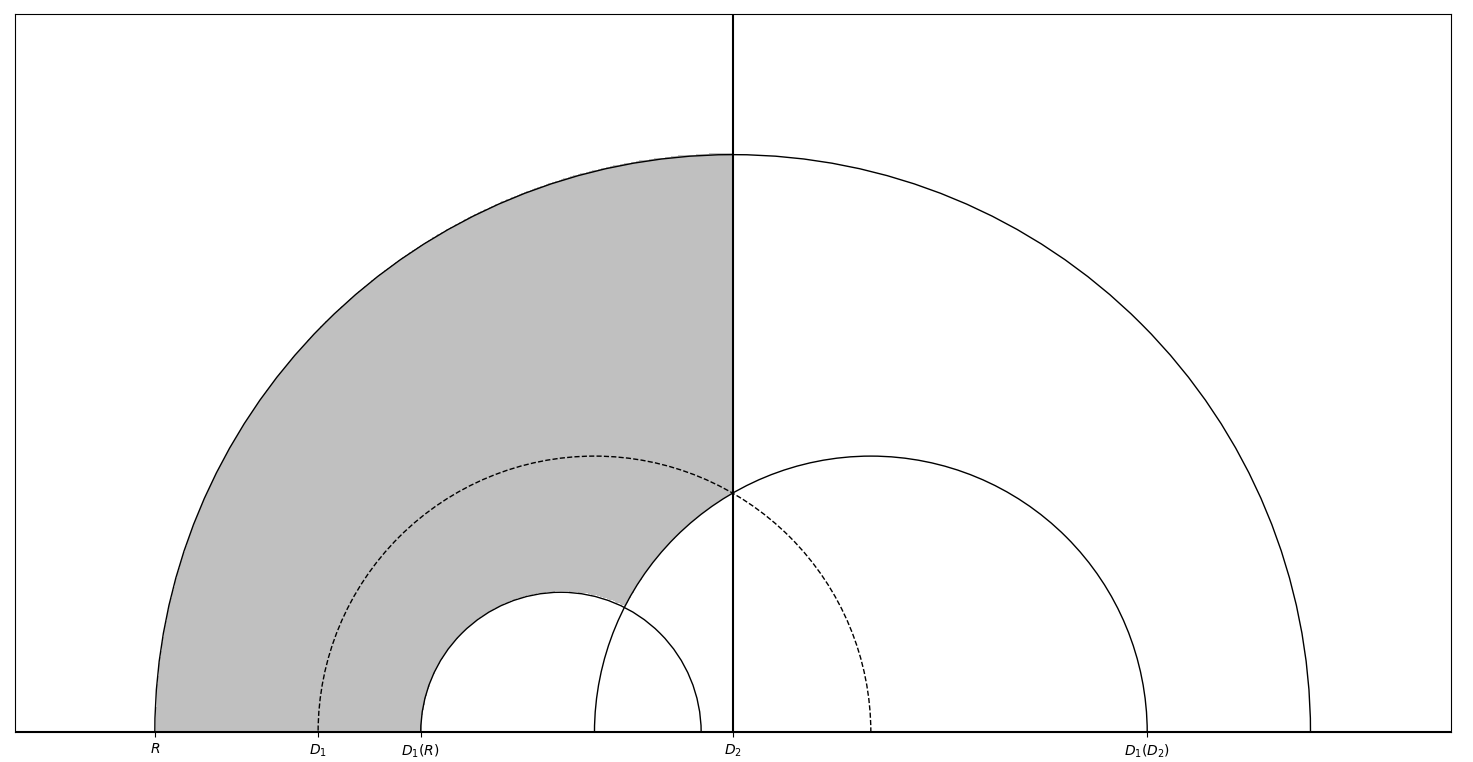
\includegraphics[width=0.7\linewidth]{doubled_cover_UHP.png}
	\caption{Fundamental Domain in the upper half plane model for $C^{-1}\Gamma_0C$ with $\theta = \pi/2$}
	\label{fd_doubled_UHP}
\end{figure}

\subsection*{A Flare Domain for $\Gamma_0$}

Next, we want to use the flare present in $\Gamma_0$'s fundamental domain to map over to a flare domain (see Appendix A for a definition).
Recall that in flare domains, we have a Fourier expansion for Maass forms in polar coordinates.

Our first step for mapping to a flare domain is to identify the matrix in $\Gamma_0$ whose axis\footnote{Recall that the \textit{axis} of a hyperbolic matrix is the geodesic whose endpoints are the fixed points of the matrix.} cuts off the flare.
In reflection groups, these tend to be easy to identify by composing reflections involving the geodesics which define the flare.
In the case of $\Gamma_0$, one quickly recognizes $D_1R$ to be the appropriate transformation (see Figures \ref{cover_with_flare} and \ref{cover_with_flare_UHP} for geometric verification).
\begin{figure}
	\centering
	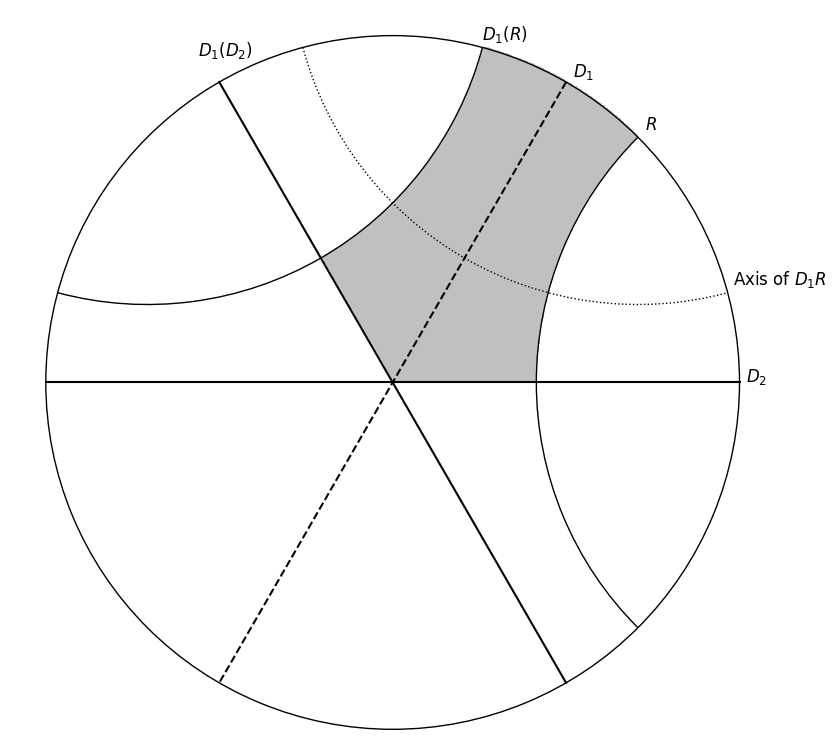
\includegraphics[width=0.5\linewidth]{cover_with_flare.png}
	\caption{Axis of $D_1R$ cuts off the flare}
	\label{cover_with_flare}
\end{figure}
\begin{figure}
	\centering
	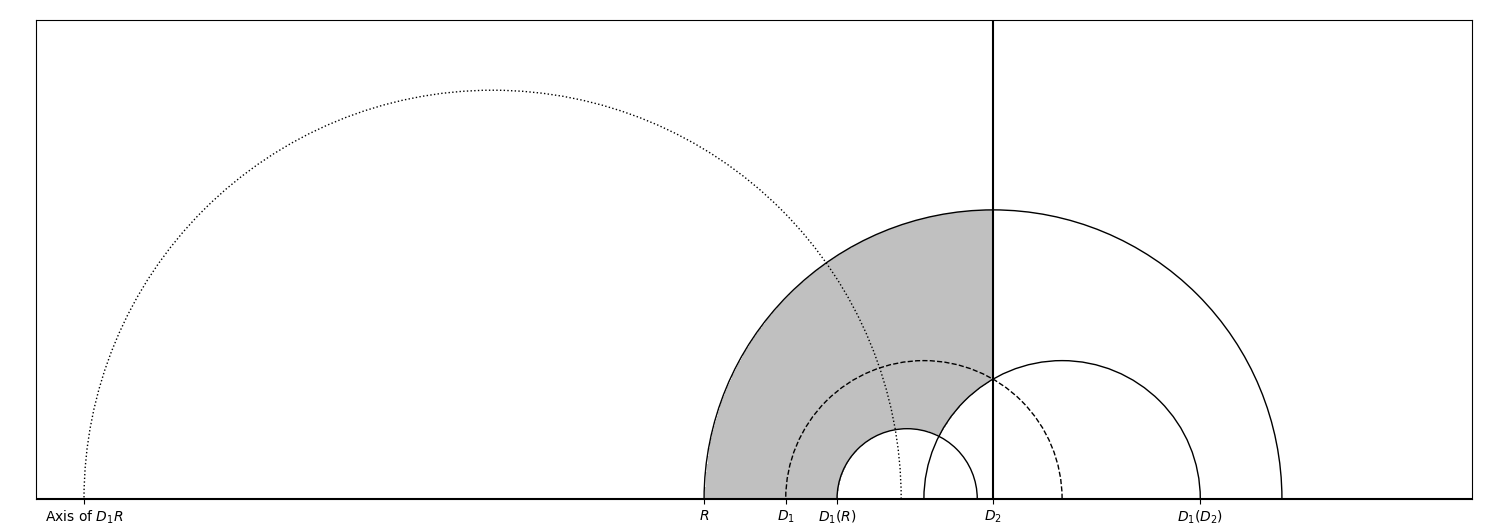
\includegraphics[width=\linewidth]{cover_with_flare_UHP.png}
	\caption{Axis of $D_1R$ cuts off the flare}
	\label{cover_with_flare_UHP}
\end{figure}

In matrix form, one finds that
$$
D_1R =
\frac{1}{2}
\begin{pmatrix}
-\sqrt{3} + i\csc\frac{\theta}{2} & \sqrt{3} - i\cot\frac{\theta}{2} \\
\sqrt{3} + i\cot\frac{\theta}{2} & -\sqrt{3} - i\csc\frac{\theta}{2}
\end{pmatrix}
$$
In the upper half plane model, this is
$$
C^{-1}D_1RC =
\frac{1}{2}
\begin{pmatrix}
-\sqrt{3}\tan\frac{\theta}{4} & \cot\frac{\theta}{4} \\
-\tan\frac{\theta}{4} & -\sqrt{3}\cot\frac{\theta}{4}
\end{pmatrix}
$$

In particular, we can utilize the flare in the upper half plane model to map over to a flare domain (again, see Appendix A for a discussion of this map).
Letting $z_1 < z_2$ be the endpoints of the axis defined by $D_1R$ (in the upper half plane model), and letting $t$ be the left end point of $R$ (again, in $\mathbb{H}$), we apply the map
$$
U(z) = \left( \frac{t - z_2}{t - z_1} \right) \frac{z - z_1}{z - z_2}
$$
to our fundamental domain and end up with the flare domain shown in Figure
\begin{figure}
	\centering
	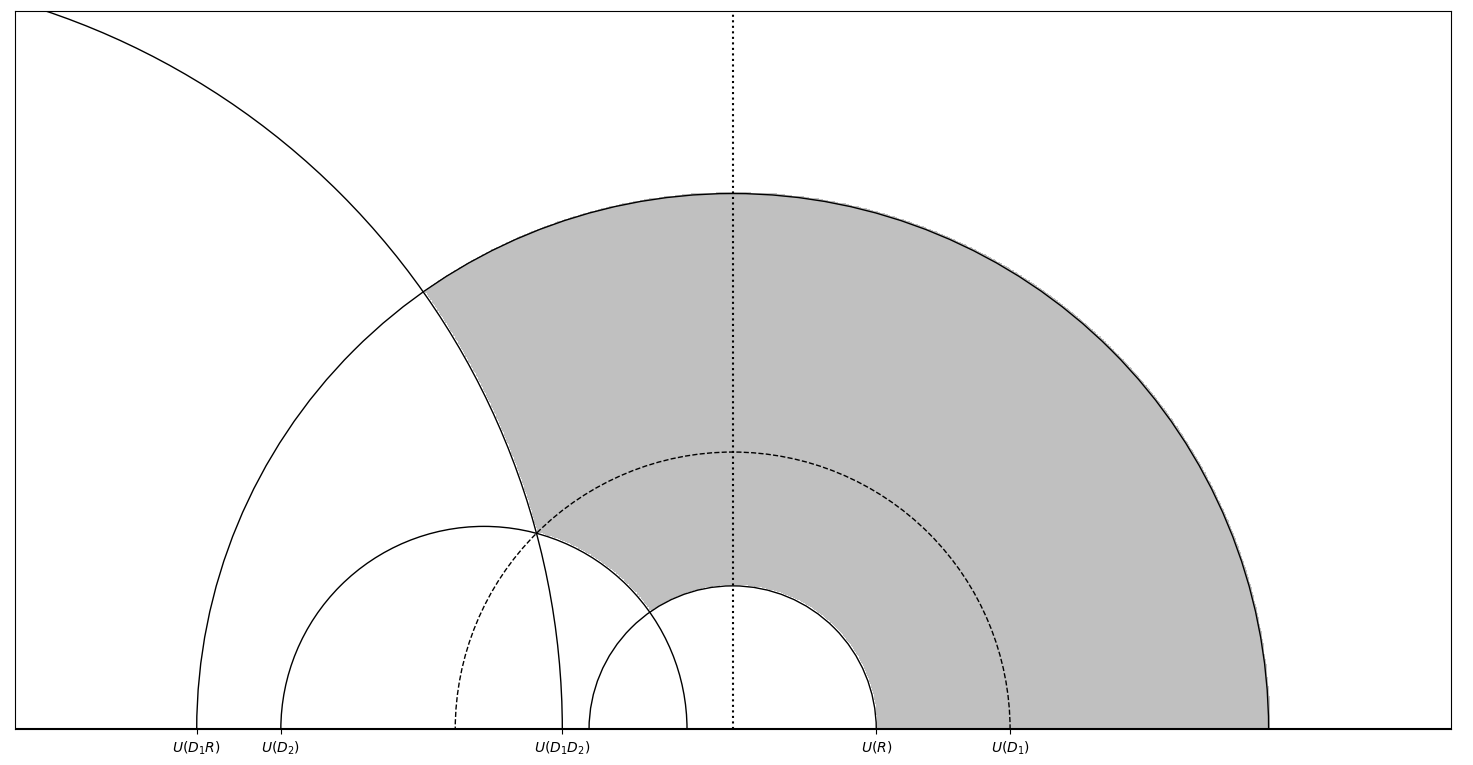
\includegraphics[width=0.7\linewidth]{cover_flare.png}
	\caption{Flare domain for the group $\Gamma_0$ with parameter $\theta = \frac{\pi}{2}$}
	\label{cover_flare}
\end{figure}

\clearpage

\section*{Appendix A: Flare Domains}

Let us look at a generic flare: two geodesics separated by positive length interval on the real line, plus a geodesic cutting through both of these at a right angle.
Let the two points on this last geodesic be labeled $z_1 < z_2$, and call the rightmost point of the first geodesic $t$.
See Figure \ref{pre_flare}.
\begin{figure}[h]
	\centering
	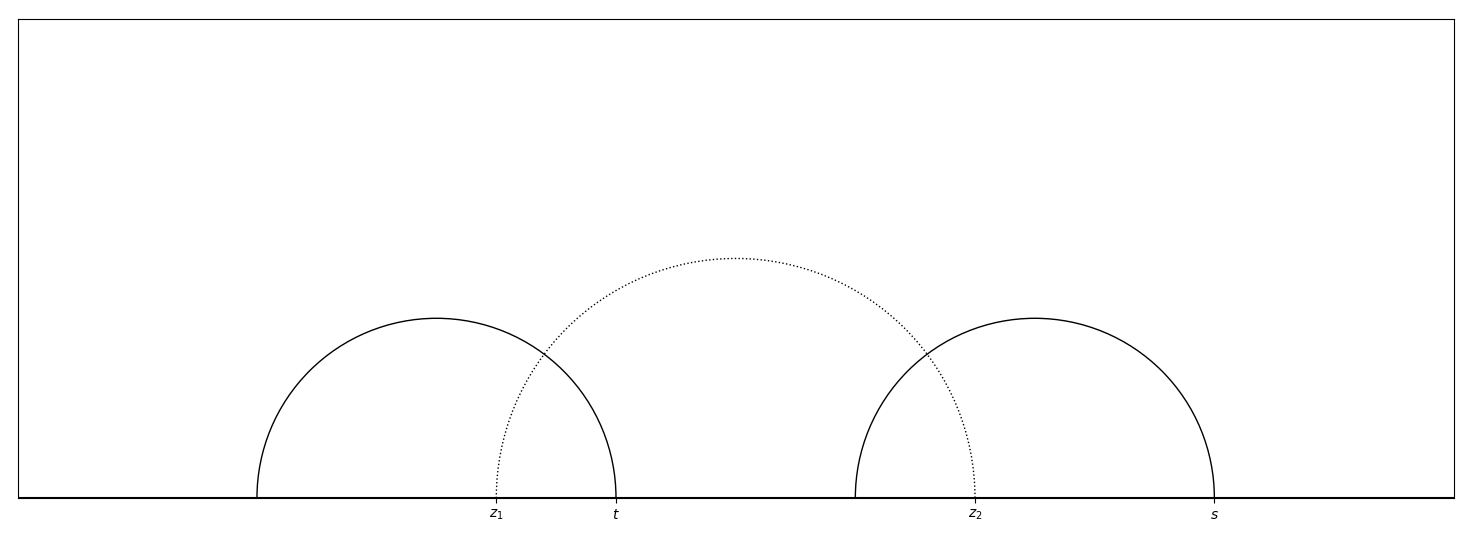
\includegraphics[width=0.6\linewidth]{labeled_pre_flare.png}
	\caption{A generic flare.}
	\label{pre_flare}
\end{figure}
Now consider the M\"obius transformation
$$
U(z) = \left( \frac{t - z_2}{t - z_1} \right) \frac{z - z_1}{z - z_2}
$$
This function is chosen so that
$$
U(z_1) = 0 ~~~~~ U(z_2) = \infty ~~~~~ U(t) = 1
$$
Thus, applying such a $U$ to a generic flare gives us a \textit{flare domain}.
See Figure \ref{post_flare} for an example.
\begin{figure}[h]
	\centering
	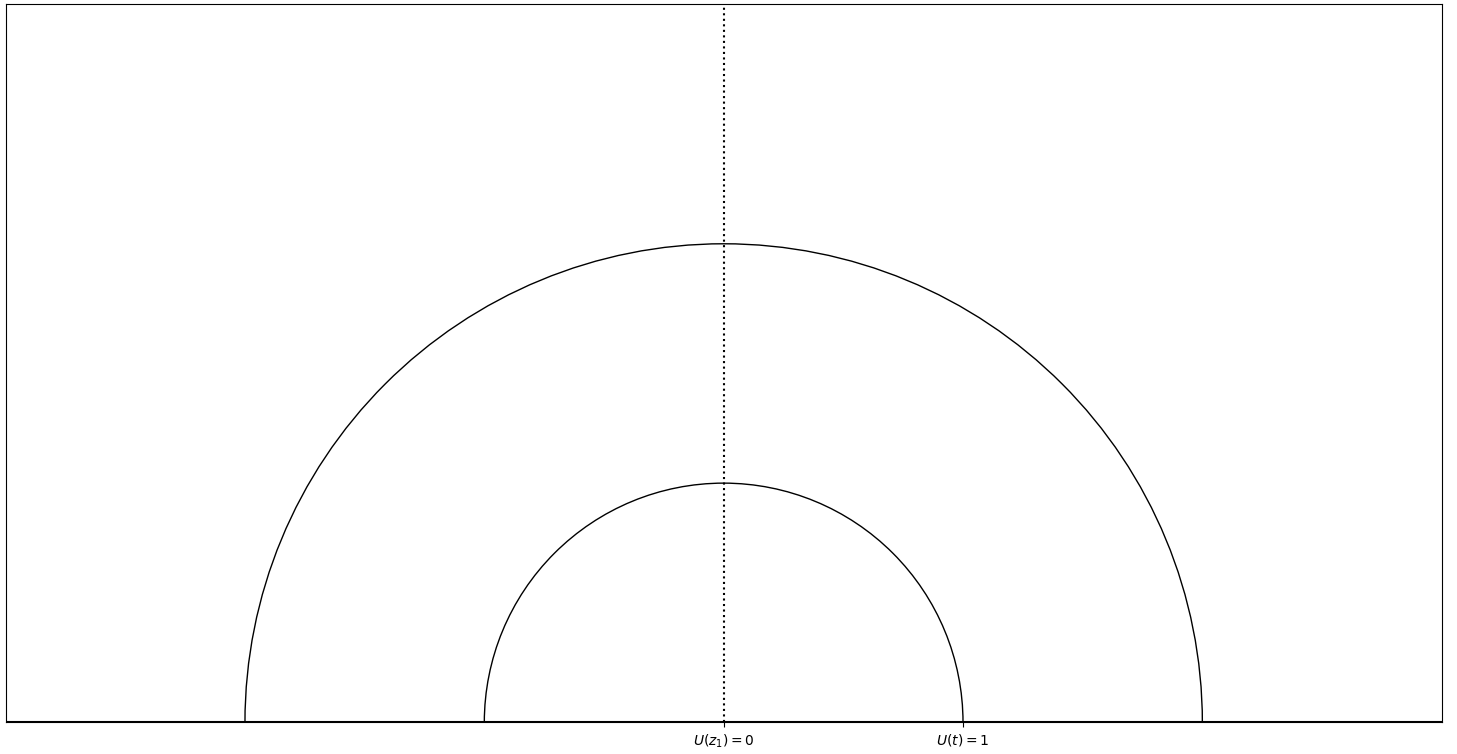
\includegraphics[width=0.6\linewidth]{labeled_flare.png}
	\caption{A flare domain.}
	\label{post_flare}
\end{figure}

\end{document}